% Created 2014-11-06 Thu 12:26
\documentclass[presentation]{beamer}
\usepackage[utf8]{inputenc}
\usepackage[T1]{fontenc}
\usepackage{fixltx2e}
\usepackage{graphicx}
\usepackage{longtable}
\usepackage{float}
\usepackage{wrapfig}
\usepackage{rotating}
\usepackage[normalem]{ulem}
\usepackage{amsmath}
\usepackage{textcomp}
\usepackage{marvosym}
\usepackage{wasysym}
\usepackage{amssymb}
\usepackage{hyperref}
\tolerance=1000
\usepackage{CJK}
\usepackage{indentfirst}
\usepackage[pdftex]{graphicx}
\usepackage{fancyhdr}
\usepackage[CJKbookmarks=true]{hyperref}
%% Define a museincludegraphics command, which is
%%   able to handle escaped special characters in image filenames.
\def\museincludegraphics{%
  \begingroup
  \catcode`\|=0
  \catcode`\\=12
  \catcode`\#=12
  \includegraphics[width=0.75\textwidth]
}
\usetheme{default}
\author{Heyan Huang}
\date{\today}
\title{CS120 Lab \alert{10} Section \alert{6}}
\hypersetup{
  pdfkeywords={},
  pdfsubject={},
  pdfcreator={Emacs 24.3.1 (Org mode 8.2.7c)}}
\begin{document}

\maketitle

\begin{frame}[label=sec-1]{Quiz for Week 9 \alert{Answers}}
\begin{block}{(3 pts) Perform the following base conversions:}
0010 1110 binary to decimal
\begin{itemize}
\item 1$_{\text{3}}$ 1$_{\text{2}}$ 0$_{\text{1}}$ 1$_{\text{0}}$
\end{itemize}

= 1*2$^{\text{3}}$ + 1*2$^{\text{2}}$ + 0*2$^{\text{1}}$ + 1*2$^{\text{0}}$

= 8 + 4 + 0 + 1 

= (13)$_{\text{10}}$
\\
\begin{itemize}
\item 0$_{\text{7}}$ 0$_{\text{6}}$ 1$_{\text{5}}$ 0$_{\text{4}}$  1$_{\text{3}}$ 1$_{\text{2}}$ 1$_{\text{1}}$ 0$_{\text{0}}$
\end{itemize}

= 0*2$^{\text{7}}$ + 0*2$^{\text{6}}$ + 1*2$^{\text{5}}$ + 0*2$^{\text{4}}$ + 1*2$^{\text{3}}$ + 1*2$^{\text{2}}$ + 1*2$^{\text{1}}$ + 0*2$^{\text{0}}$

= 0 + 0 + 32 + 0 + 8 + 4 + 2 + 0

= (46)$_{\text{10}}$
\end{block}
\end{frame}

\begin{frame}[label=sec-2]{Quiz for Week 9 \alert{Answers} (continued)}
38 decimal to binary
\begin{itemize}
\item (25)$_{\text{10}}$
\end{itemize}
25/2 = 12 + \alert{1}  --- 1$_{\text{0}}$

12/2 = 6 + \alert{1}   --- 1$_{\text{1}}$

6/2 = 3 + \alert{0}    --- 0$_{\text{2}}$

3/2 = 1 + \alert{1}    --- 1$_{\text{3}}$

1/2 = 0 + \alert{1}    --- 1$_{\text{4}}$

(1 1011)$_{\text{2}}$
\begin{itemize}
\item (38)$_{\text{10}}$
\end{itemize}
38/2 = 19 + \alert{0}  ---0$_{\text{0}}$

19/2 = 9 + \alert{1}   ---1$_{\text{1}}$

9/2 = 4 + \alert{1}    ---1$_{\text{2}}$

4/2 = 2 + \alert{0}    ---0$_{\text{3}}$

2/2 = 1 + \alert{0}    ---0$_{\text{4}}$

1/2 = 0 + \alert{1}    ---1$_{\text{5}}$

(10 0110)$_{\text{2}}$
\end{frame}

\begin{frame}[label=sec-3]{Quiz for Week 9 \alert{Answers} (continued)}
A3 Hex to decimal
\begin{itemize}
\item (E$_{\text{2}}$ 4$_{\text{1}}$ 2$_{\text{0}}$)$_{\text{16}}$
\end{itemize}
= E*16$^{\text{2}}$ + 4*16$^{\text{1}}$ + 2*16$^{\text{0}}$

= 14*256 + 4*16 + 2$_{\text{0}}$

= 3584 + 64 + 2

= 3650 
\begin{itemize}
\item (A$_{\text{1}}$ 3$_{\text{0}}$)$_{\text{16}}$
\end{itemize}
= A*16$^{\text{1}}$ + 3*16$^{\text{0}}$

= 10*16 + 3*1

= (163)$_{\text{10}}$
\end{frame}

\begin{frame}[fragile,label=sec-4]{Quiz for Week 9 \alert{Answers} (continued)}
 (2 pts) Write the statements necessary to initialize the array declared below to ascending even numbers starting at 0. That is, a[ 0 ] should be 0, a[ 1 ] should be 2, a[ 2 ] should be 4, etc\ldots{}
\begin{verbatim}
int a[ 850 ];
\end{verbatim}
\begin{verbatim}
for (int i = 0; i < 850; ++i) {
    a[i] = i * 2;
}  

for (int i = 0; i <= 849; ++i) {
    a[i] = i * 2;
}  

int j = 0;
for (int i = 0; i <= 849; ++i) {
    a[i] = j;
    j += 2;
}
\end{verbatim}
\end{frame}

\begin{frame}[fragile,label=sec-5]{Function Call Process}
 \begin{verbatim}
#include <stdio.h>

int b();
int c();

int a() {
    b();
    c();
    return 0;
}
int b() { return 0; }
int c() { return 0; }

int main() {
    a();
    return 0;
}
\end{verbatim}
\end{frame}

\begin{frame}[label=sec-6]{Function Call Process}
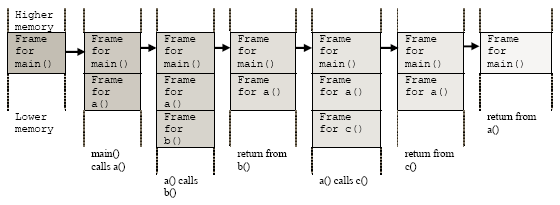
\includegraphics[width=.9\linewidth]{./func.png}
\end{frame}

\begin{frame}[label=sec-7]{Pass-by-Value}
\begin{center}
\begin{tabular}{lll}
\hline
int main() \{ &  & int foo(int z) \{\\
int x = 7; &  & int a;\\
int y; &  & a = z + 5;\\
y = foo(x); & 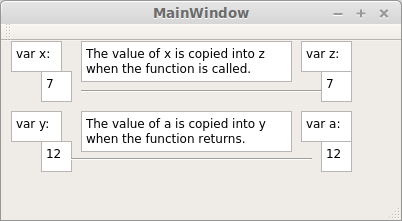
\includegraphics[width=.4\linewidth]{./myfunc.png} & return a;\\
\} &  & \}\\
\alert{main() \& its variables} &  & \alert{foo() \& its variables}\\
\hline
\end{tabular}
\end{center}
\end{frame}

\begin{frame}[label=sec-8]{Pass-by-Reference}
\begin{center}
\begin{tabular}{lll}
\hline
int main() \{ &  & int foo(int \&z) \{\\
int x = 7; &  & int a;\\
int y; &  & a = z + 5;\\
y = foo(x); & 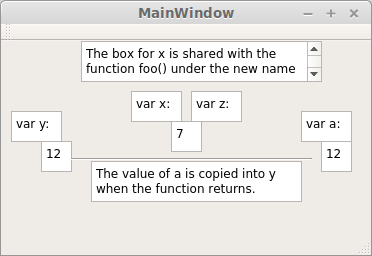
\includegraphics[width=.4\linewidth]{./reference.png} & return a;\\
\} &  & \}\\
\alert{main() \& its variables} &  & \alert{foo() \& its variables}\\
\hline
\end{tabular}
\end{center}
\end{frame}

\begin{frame}[label=sec-9]{Array: Pass-by-Reference}
\begin{center}
\begin{tabular}{lll}
\hline
int main() \{ &  & int foo(int z[]) \{\\
int numbers[ 10 ]; &  & \\
numbers[ 0 ] = 0; &  & z[ 2 ] = 88;\\
numbers[ 1 ] = 1; &  & \\
foo(numbers); & 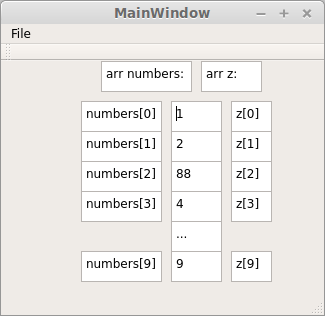
\includegraphics[width=.4\linewidth]{./array.png} & \\
\} &  & \}\\
\alert{main() \& its variables} &  & \alert{foo() \& its variables}\\
\hline
\end{tabular}
\end{center}
\end{frame}

\begin{frame}[label=sec-10]{Scores of Quiz Week 9 and Lab 8}
\\
\begin{itemize}
\item \alert{Quiz for Week 9} Distribution:
\end{itemize}
\begin{center}
\begin{tabular}{lrrrrrrr}
\hline
Score & 0 & 1 & 2 & 3 & 4 & 5 & Missed\\
\hline
Section \alert{4} Count (22) & 2 & 2 & 2 & 5 & 3 & 3 & 5\\
\hline
Section \alert{6} Count (24) &  & 2 & 7 & 3 & 2 & 1 & 9\\
\hline
\end{tabular}
\end{center}
\\
\begin{itemize}
\item \alert{Lab 8}:
\end{itemize}
\begin{center}
\begin{tabular}{lrrrrrrr}
\hline
Score & <9 & 9 & 10 & 11 & 12 & 13 & Missed\\
\hline
Section \alert{4} Count (22) & 2 &  & 3 & 1 & 2 & 5 & 9\\
\hline
Section \alert{6} Count (24) &  & 2 & 2 &  & 6 & 4 & 10\\
\hline
\end{tabular}
\end{center}
\\
\begin{itemize}
\item \alert{Lab 9}:
\begin{itemize}
\item Will hand it back during coming lab
\end{itemize}
\end{itemize}
\end{frame}

\begin{frame}[label=sec-11]{Lab 10 Specific Requirements}
\begin{itemize}
\item \alert{cscheckin}:
\begin{itemize}
\item \alert{Source Programs} only: \alert{Lab10Sec6.cpp}
\end{itemize}
\end{itemize}
\\
\begin{itemize}
\item \alert{Hard Copy}:
\begin{itemize}
\item \alert{Source Program}: 
\begin{itemize}
\item Lab10Sec6.cpp
\end{itemize}
\item \alert{Script Output} of the program
\end{itemize}
\end{itemize}
\end{frame}
% Emacs 24.3.1 (Org mode 8.2.7c)
\end{document}